\section{Internet of Things}
\label{sec:IoT}
O termo \textit{Internet of Things} foi usado pela primeira vez pelos fundadores do \textit{MIT Auto-ID Center},
mencionado especialmente pelo britânico Kevin Ashton no ano de 1999, referindo-se especificamente a área de
Gerenciamento da Cadeia de Suprimentos~\cite{kevinashton2009}. Com o passar do tempo, as aplicações utilizando
esse conceito se ampliaram, sendo aplicadas em áreas como transporte, cuidados com a saúde, automação residencial,
entre outras. Devido a essa evolução no paradigma, a definição de \textit{Things} foi se tornando cada vez mais
abrangente, representando desde implantes de monitoramento cardíacos e transponders para identificação animal
até automóveis com sensores integrados, sensores para análise de luminosidade e temperatura.
A \textit{Internet of Things} consiste basicamente em uma rede de objetos físicos (\textit{Things}) que fornecem
informações específicas de seu contexto, gerando assim, uma enorme quantidade de dados desconexos que precisam
ser armazenados, processados e apresentados de uma forma eficiente e de fácil interpretação. O grande valor
encontrado no conceito de \textit{Internet of Things} é relação das informações produzida por essa rede de
dispositivos.

\subsection{Aplicações}
Com a facilitação do acesso e integração de uma grande variedade de dispositivos heterogêneos, uma série de
áreas distintas começou a obter vantagens do paradigma, aplicando interpretações dentro de seu contexto
das informações recebidas para criar soluções para seus respectivos problemas.

\label{sec:IoTAp}
\subsubsection{Smart City}
Além das barreiras técnicas, a adoção do paradigma de \textit{Internet of Things} também é prejudicado
pela dificuldade na criação de um modelo de negócio claro e amplamente aceito para atrair investidores
a financiar o desenvolvimento destas tecnologias~\cite{RePEc:zbw:itse13:88475}.
Neste cenário complexo, a aplicação do conceito de \textit{Internet of Things} em um ambiente urbano
pode se tornar particularmente interessante por atender à forte intenção de muitos governos de adotar
soluções TIC (Tecnologias da Informação e Comunicação) para administração pública.
Apesar de não haver uma definição formal amplamente aceita de \textit{Smart City}, a intenção final é de
alcançar uma melhor utilização dos recursos públicos, oferecendo uma melhor qualidade nos serviços oferecidos
aos cidadãos ao mesmo tempo em que reduz os custos operacionais da administração pública~\cite{IoTSmart2014}.
Este objetivo pode ser atingido pela utilização de um \textit{IoT} urbano, como por exemplo uma infraestrutura
para controlar a utilização de iluminação pública baseada no clima ou sensores em latas de lixo para
identificar a melhor rota para seu recolhimento com base em sua utilização. Grandes empresas como a
IBM e a GE tem investido muito nessa área, criando pilotos bem sucedidos de \textit{Smart City}.

\subsubsection{Automação Residencial}
Há atualmente um vasto leque de soluções inteligentes para automação residencial. Desde 

\subsubsection{Sistemas Médicos e de Saúde Pessoal}
Uma das áreas de aplicação mais proeminente é a relacionada à saúde. Atualmente existem muitas aplicações
de IoT com o intuito de melhorar a saúde pessoal baseadas em dados como exercícios físicos realizados,
análise da qualidade do sono e alimentação. Grandes empresas como a Apple estão investindo fortemente nessa
área e tornando-a cada vez mais fértil com a criação de novos sensores e interligação de dados.
Ainda dentro da área da saúde, existem aplicações com foco maior na área médica, como, por exemplo,
avaliação de pacientes a distância, possibilitando um atendimento mais rápido e específico baseados em uma
série de informações provenientes de sensores com finalidades distintas como pressão sangüinea,
frequência cardíaca, temperatura entre outros. Essas aplicações representam um grande avanço, tendo
em vista que pela primeira vez, é possível acessar informações precisas em tempo real, além de possibilitar
a montagem de grupos de teste com uma facilidade sem precedentes. Essa área se tornou tão proeminente que
possui uma terminologia própria, \textit{IoMT} (\textit{Internet of Medical Things}).


\subsection{Plataformas para IoT Existentes}
\label{sec:IoTPlataformas}

\subsubsection{mbed}
A empresa ARM provê uma solução completa de \textit{Internet of Things} (IoT) chamada mbed\cite{mbed}.
Esta plataforma é dividida em três módulos, mbed OS, mbed Device Server e mbed Tools.\\
A plataforma utiliza em seu sistema embarcado a tecnologia mbedTLS para criptografia de dados com baixo
consumo de memória, desenvolvida inicialmente sob o nome de PolarSSL pela empresa holandesa Offspark,
que foi comprada recentemente pela ARM.

\subsubsubsection{mbed OS}
É um sistema operacional, disponibilizado de graça, para processadores da linha ARM Cortex-M, que são
desenvolvidos visando a eficiência de energia e produtividade.\\
A arquitetura do mbed OS fornece componentes de software e um framework de aplicação que, combinados
com a grande diversidade de empresas e desenvolvedores que disponibilizam bibliotecas e drivers, facilitam
e agilizam o processo de desenvolvimento de aplicações para IoT.\\
O mbed OS provê suporte aos padrões como Bluetooth Smart®, Cellular, Thread, Wi-Fi®, e 802.15.4/6LoWPAN junto
com TLS/DTLS, CoAP, HTTP, MQTT e Lightweight M2M

\subsubsubsection{mbed Device Server}
É um produto que precisa de licença, serve para conectar e gerenciar os dispositivos de uma forma segura.
Ele provê a ligação entre os os protocolos utilizados nos dispositivos IoT e a API que é utilizada por
desenvolvedores web. Isto simplifica a integração de dispositivos IoT que geram \lq little data\rq\ que vão
para os servidores que analizam e agregam a informação gerando a \lq big data\rq.\\
O Device Server é escalável, podendo conectar e gerenciar milhões de dispositivos.

\subsubsubsection{Arquitetura}
https://mbed.org/technology/device-server/ \\

\begin{center}
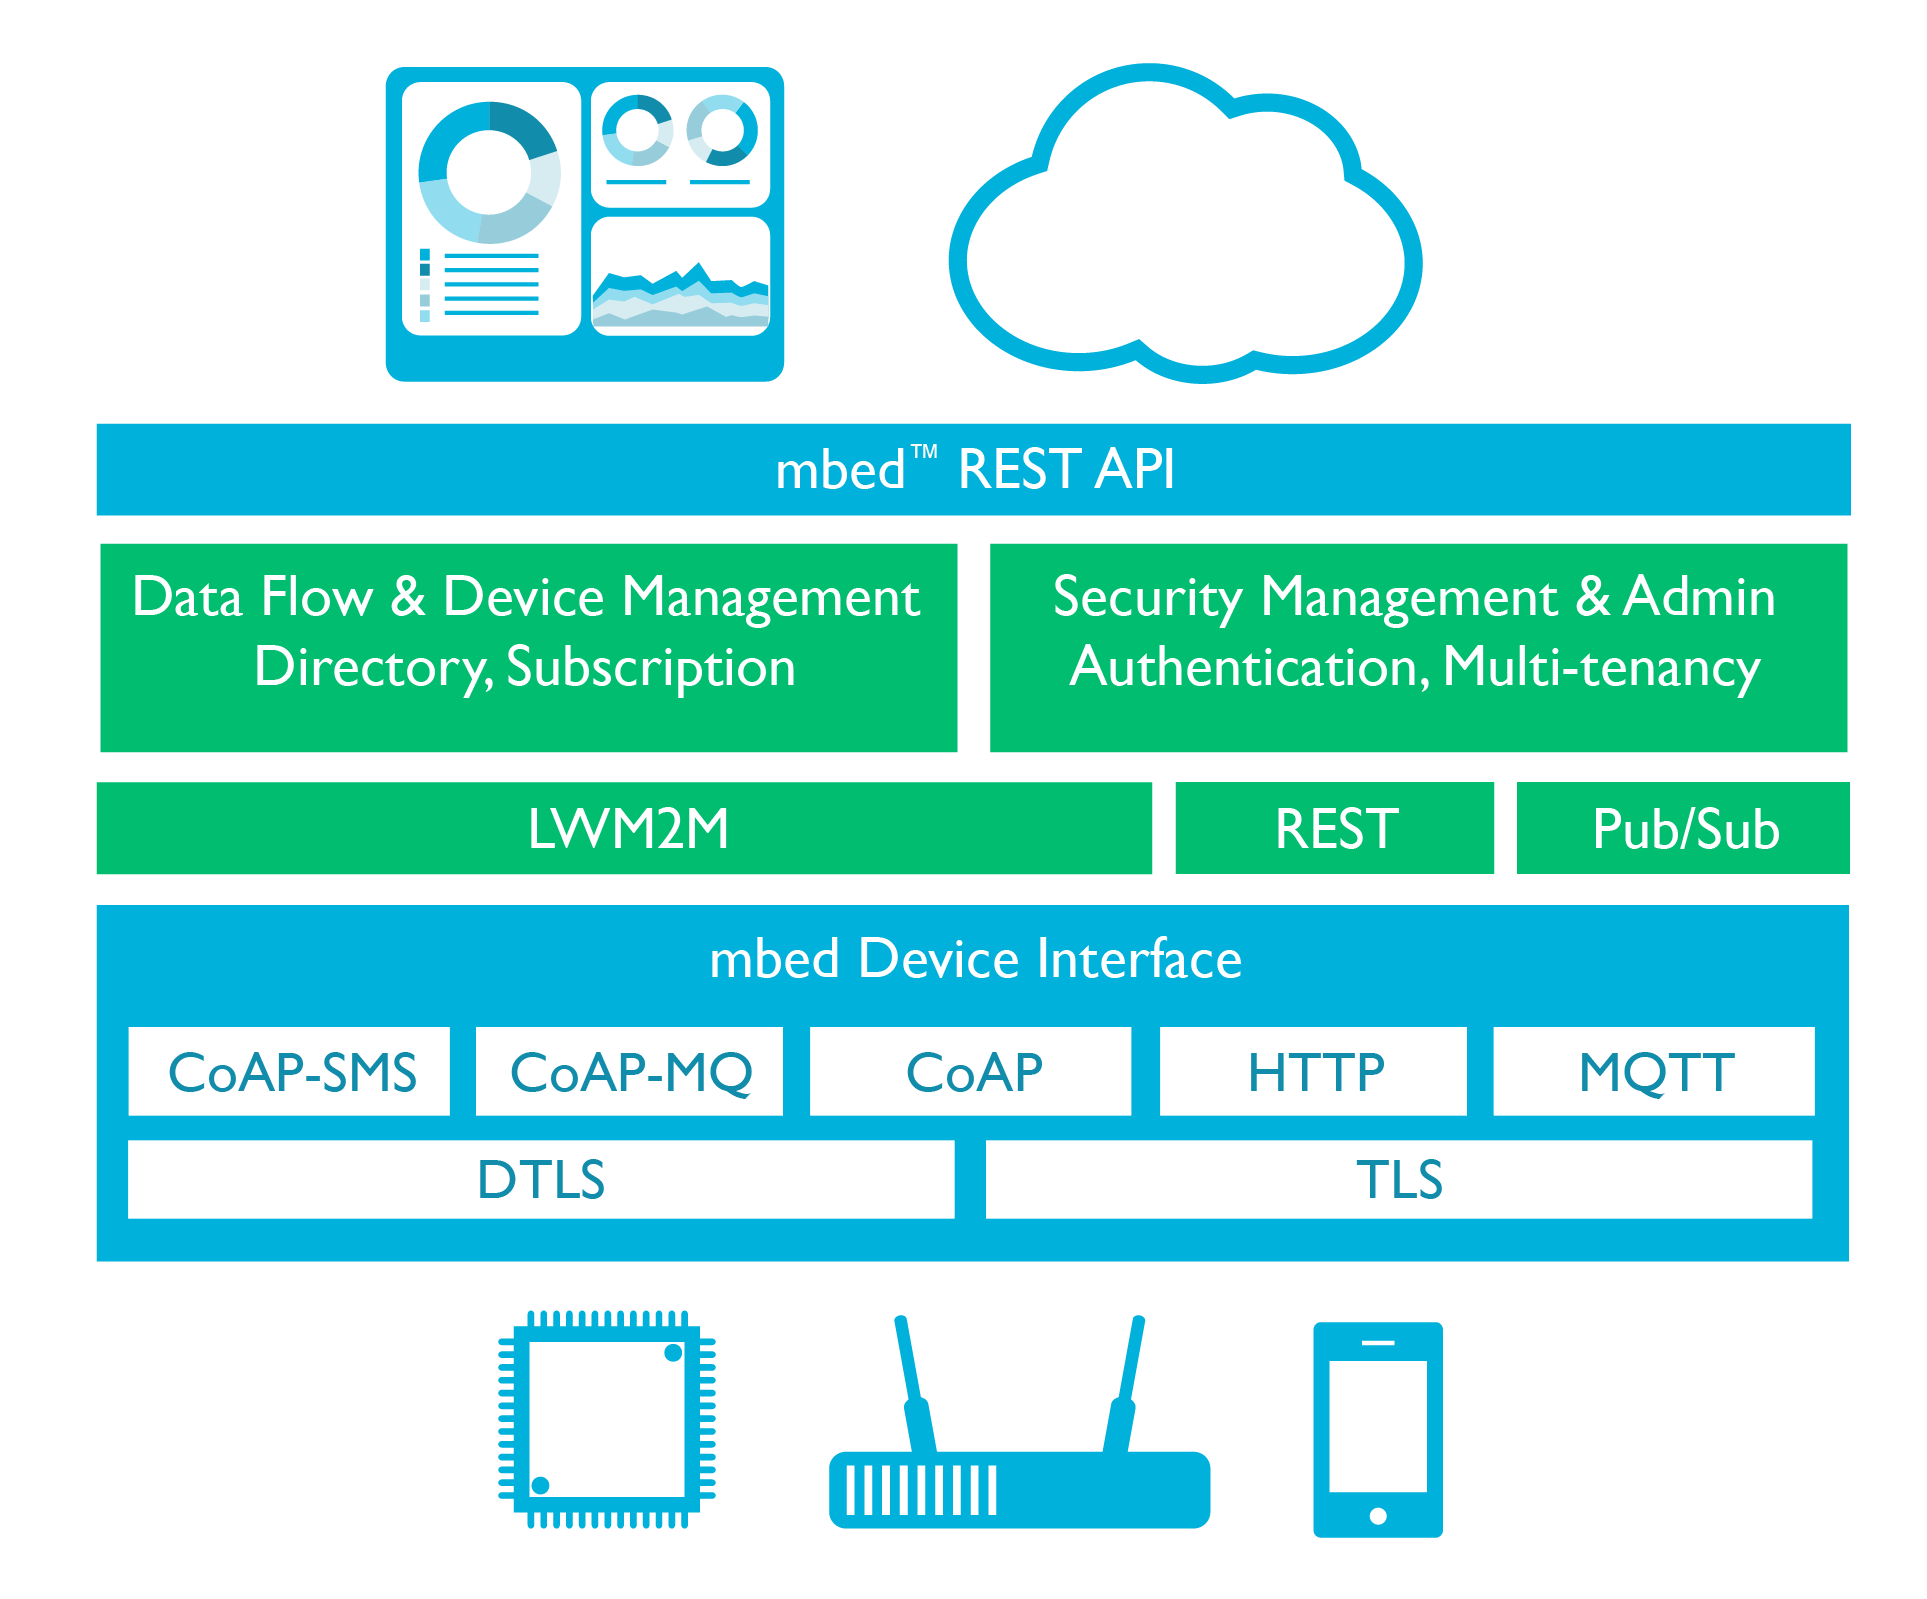
\includegraphics[width=0.5\textwidth]{fig/mbed_arch.png}
\end{center}

\subsubsection{FlowCloud}
FlowCloud~\cite{flowcloud} é uma tecnologia que visa conectar dispositivos a internet de modo a facilitar o
desenvolvimento e grernciamento de aplicações \lq machine to machine\rq\ (M2M) e \lq man to machine\rq. A imgtec,
empresa que desenvolveu o FlowCloud, visa suprir as necessidades da IoT, provendo meios de conectar dispositivos
que estão separados grograficamente estabelecendo uma conexão ponto a ponto (P2P) entre os dispositivos.

\subsubsection{Arrayent}
Arrayent~\cite{arrayent} é uma plataforma IoT que oferece conexão e segurança entre dispositivos IoT e aplicações
para  smartphones, tablets e web com baixo custo e simplicidade. A plataforma é composta de 4 componentes:
Arrayent Connect Agent, Arreyent Connect Cloud, Arrayent Mobile Framework e Arrayent Cloud Insight.

\subsubsubsection{Arrayent Connect Agent}
É utilizado por desenvolvedores de softare embarcado. Funciona como um módulo do firmware que gerencia a
seção do dispositivo com junto ao Arreyent Connect Cloud e abstrai essa responsabilidade para o desenvolvedor
do firmware, deixando-o livre para se preocupar em desenvolver apenas as funcionalidades necessárias para o
funcionamento do dispositivo.\\
Atualmente ele suporta Wi-Fi, ZigBee, Z-Wave LAN e os sistemas operacionais Linux ou FreeRTOS.

\subsubsubsection{Arrayent Connect Cloud}
O Arrayent Connect Cloud é o coração da plataforma de IoT da Arrayent. Ele é essencialmente um sistema
operacional baseado na cloud que agrega os dispositivos virtualizados, que são uma cópia dos dispositivos
físicos, para que as aplicações web e mobile possam se conectar e recolher informações ou executar comandos
sobre os dispositivos. Além disso, o Arreyent Connect Cloud pode emitir alertas, fazer update de firmware
\lq over-the-air\rq, gerenciar contas de usuários e muito mais.

\subsubsubsection{Arreyent Mobile Framework}
O Arrayent Mobile Framework ajuda os desenvolvedores mobile a criar rapidamente aplicativos intuitivos e
confiáveis para o mercado. Ele abstrai a complexidade envolvida na utilização da plataforma M2M da Arrayent,
que é uma API web de baixo nível, deixando o desenvolvedor livre para se preocupar apenas com as funcionalidades
e beleza dos aplicativos por ele desenvolvidos.

\subsubsubsection{Arrayent Cloud Insight}
O Arrayent Cloud Insight é responsável pela camada de negócio, fornecendo serviços de Business Intelligence,
gerando relatórios de dados comuns a todos os seus produtos como localização do dispositivo, interações entre
os dispositivos e as aplicações, tendência de pico de utilização e muito mais. O Arrayent Cloud Insight agrega,
normaliza, filtra e entrega os dados dos dispositivos para qualquer solução de análise que você utilizar.

\subsubsection{Samsung IoT Plataform}
A plataforma IoT da samsung provê uma conexão padronizada de diversos dispositivos a um dispositivo
\lq smart\rq\ ou hub. A samsung disponibliza um SDK que simplifica o desenvolvimento de novos serviços, coletando
e processando os dados de sensores e serviços que o usuário possa ter. Os desenvolvedores não precisam analisar ou
fazer setup da infraestrutura complexa de conexão entre os dispositivos ou se preocupar com os dados do usuário na cloud.
A plataforma de IoT da samsung foi desenhada para que os desenvolvedores se consentrem apenas nas funcionalidades
dos serviços que estão sendo desenvolvidos por eles. Uma limitação do SDK da samsung é que ele é disponibilizado
apenas para a plataforma android 4.1 ou superior.

\subsubsection{IBM Internet of Things Foundation}
http://www-03.ibm.com/software/products/en/internet-of-things-foundation

\subsubsection{Carriots}
O Carriots é uma \textit{Plataform as a Service} (PaaS) desenvolvida para projetos envolvendo
\textit{Internet of Things}(IoT) e \textit{Machine to Machine}(M2M). O produto possui suporte
a uma série de dispositivos como Arduino, Rapsberry PI, Beagle Bone, Fez Cerbuino, Cubie Board
entre outros. Seu suporte é feito basicamente através de uma API REST, além de fornecer um SDK
Java para esta integração.

